\chapter{GIRAF Outline}

GIRAF is a tablet environment developed to ease communication between \glspl{guardian} and \glspl{citizen} with little or no verbal communication. Software students develop the project as a part of their bachelor project. The students work in small teams and coordinate the work between teams. The project is in collaboration with the following institutions \cite{GirafWebsite}, that act as customers in the development process.

\begin{itemize}
    \item Børnehaven Birken (Kindergarten) \cite{bhBirken}
    \item Egebakken (School) \cite{egebakken}
    \item Enterne (Home for disabled) \cite{enterne}
    \item The speech institute at Aalborg municipality
    \item Center for Autism and ADHD \cite{center_for_autism}
\end{itemize}

The project started in 2011, and each year, the students continue where the previous years students left off.

This semester started with the decision to, like previous years, run the project with the \gls{Scrum_principles}. One group was appointed \gls{PO} team and another was appointed \gls{SMT}. The \gls{PO} team had the responsibility of talking to the customer and making the product backlog. The \gls{SMT} had the responsibility of deciding and facilitate how the collaboration in the project should run, and which guidelines the groups had to follow.

\section{Current state of GIRAF}

When we started the semester, the work done by previous teams was handed over to us. In this section, we describe some of the elements of the material we got as they looked at the time of handover.

The GIRAF project has produced many different apps over the years. Most of the apps are not working, because the \glspl{devTeam} in 2017 changed the backend. They only had time to update one application to reflect the new backend, and therefore only one application called Weekplanner is working. The Weekplanner application is described in section \ref{sec:TheWeekplannerApplication}.

These problems come from different ideas, coding styles, and an incomplete mental model of the system, and has resulted in an incoherent structure of the project. Because the groups in 2017 \cite{SW608F18} changed the backend of the system, it left all applications at that time unuseable, since they were developed for an \gls{api} that no longer were accessible and the new \gls{api} where not backwards compatible. The groups in 2017 managed to re-build the weekplanner application so it where compatible with the new \gls{api}. They did not find time to re-build any other applications.

The Weekplanner app is the only app that has received updates in the last couple of years, and with this in mind, the \gls{PO} group also decided to limit our development to the Weekplanner app this year.

The Weekplanner app is a tool for showing autistic people what their plan is for the week. Each day has activities associated with it, ordered chronologically, each of them represented as a picture also called a pictogram. The state of the app from the start of 2019, can be seen in \autoref{fig:WeekPlannerPicture}.

\begin{figure}[H]
        \begin{center}
            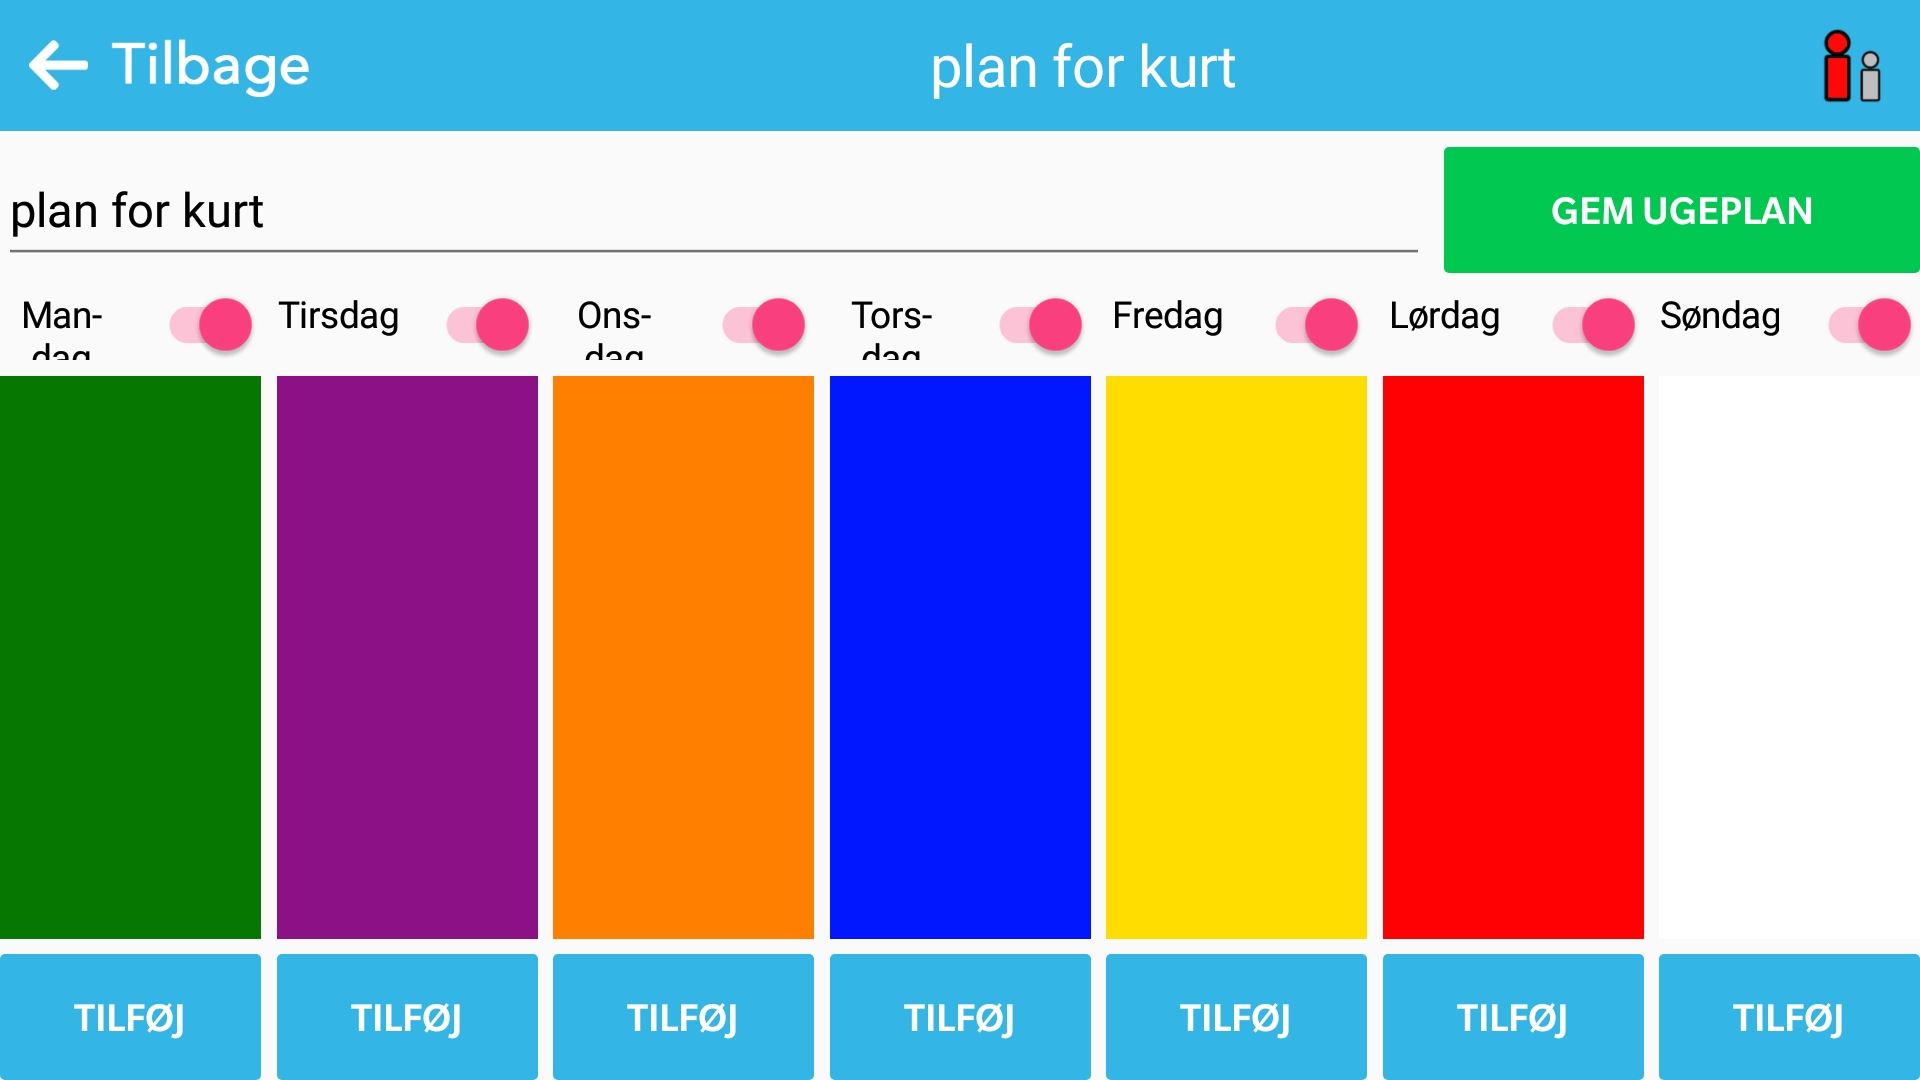
\includegraphics[width=0.95\textwidth]{figures/WeekPlannerPicture}
        \end{center}
        \caption{Weekplanner state at the start of 2019}
        \label{fig:WeekPlannerPicture}
\end{figure}

Because the customers deem the Weekplanner application as the most important application of the Giraf project, and because the Weekplanner application is the only application that has been updated in the last couple of years, \gls{PO} group decided to limit our development to the Weekplanner application exclusively.

The Weekplanner app is using the Xamarin framework and can run on both Android and IOS devices.

The backend is a .NET Core 2 project that uses traditional MVC and supports all the capabilities of the current Weekplanner app. It exposes a REST-inspired API to the front end.
\begin{figure}[H]
        \begin{center}
            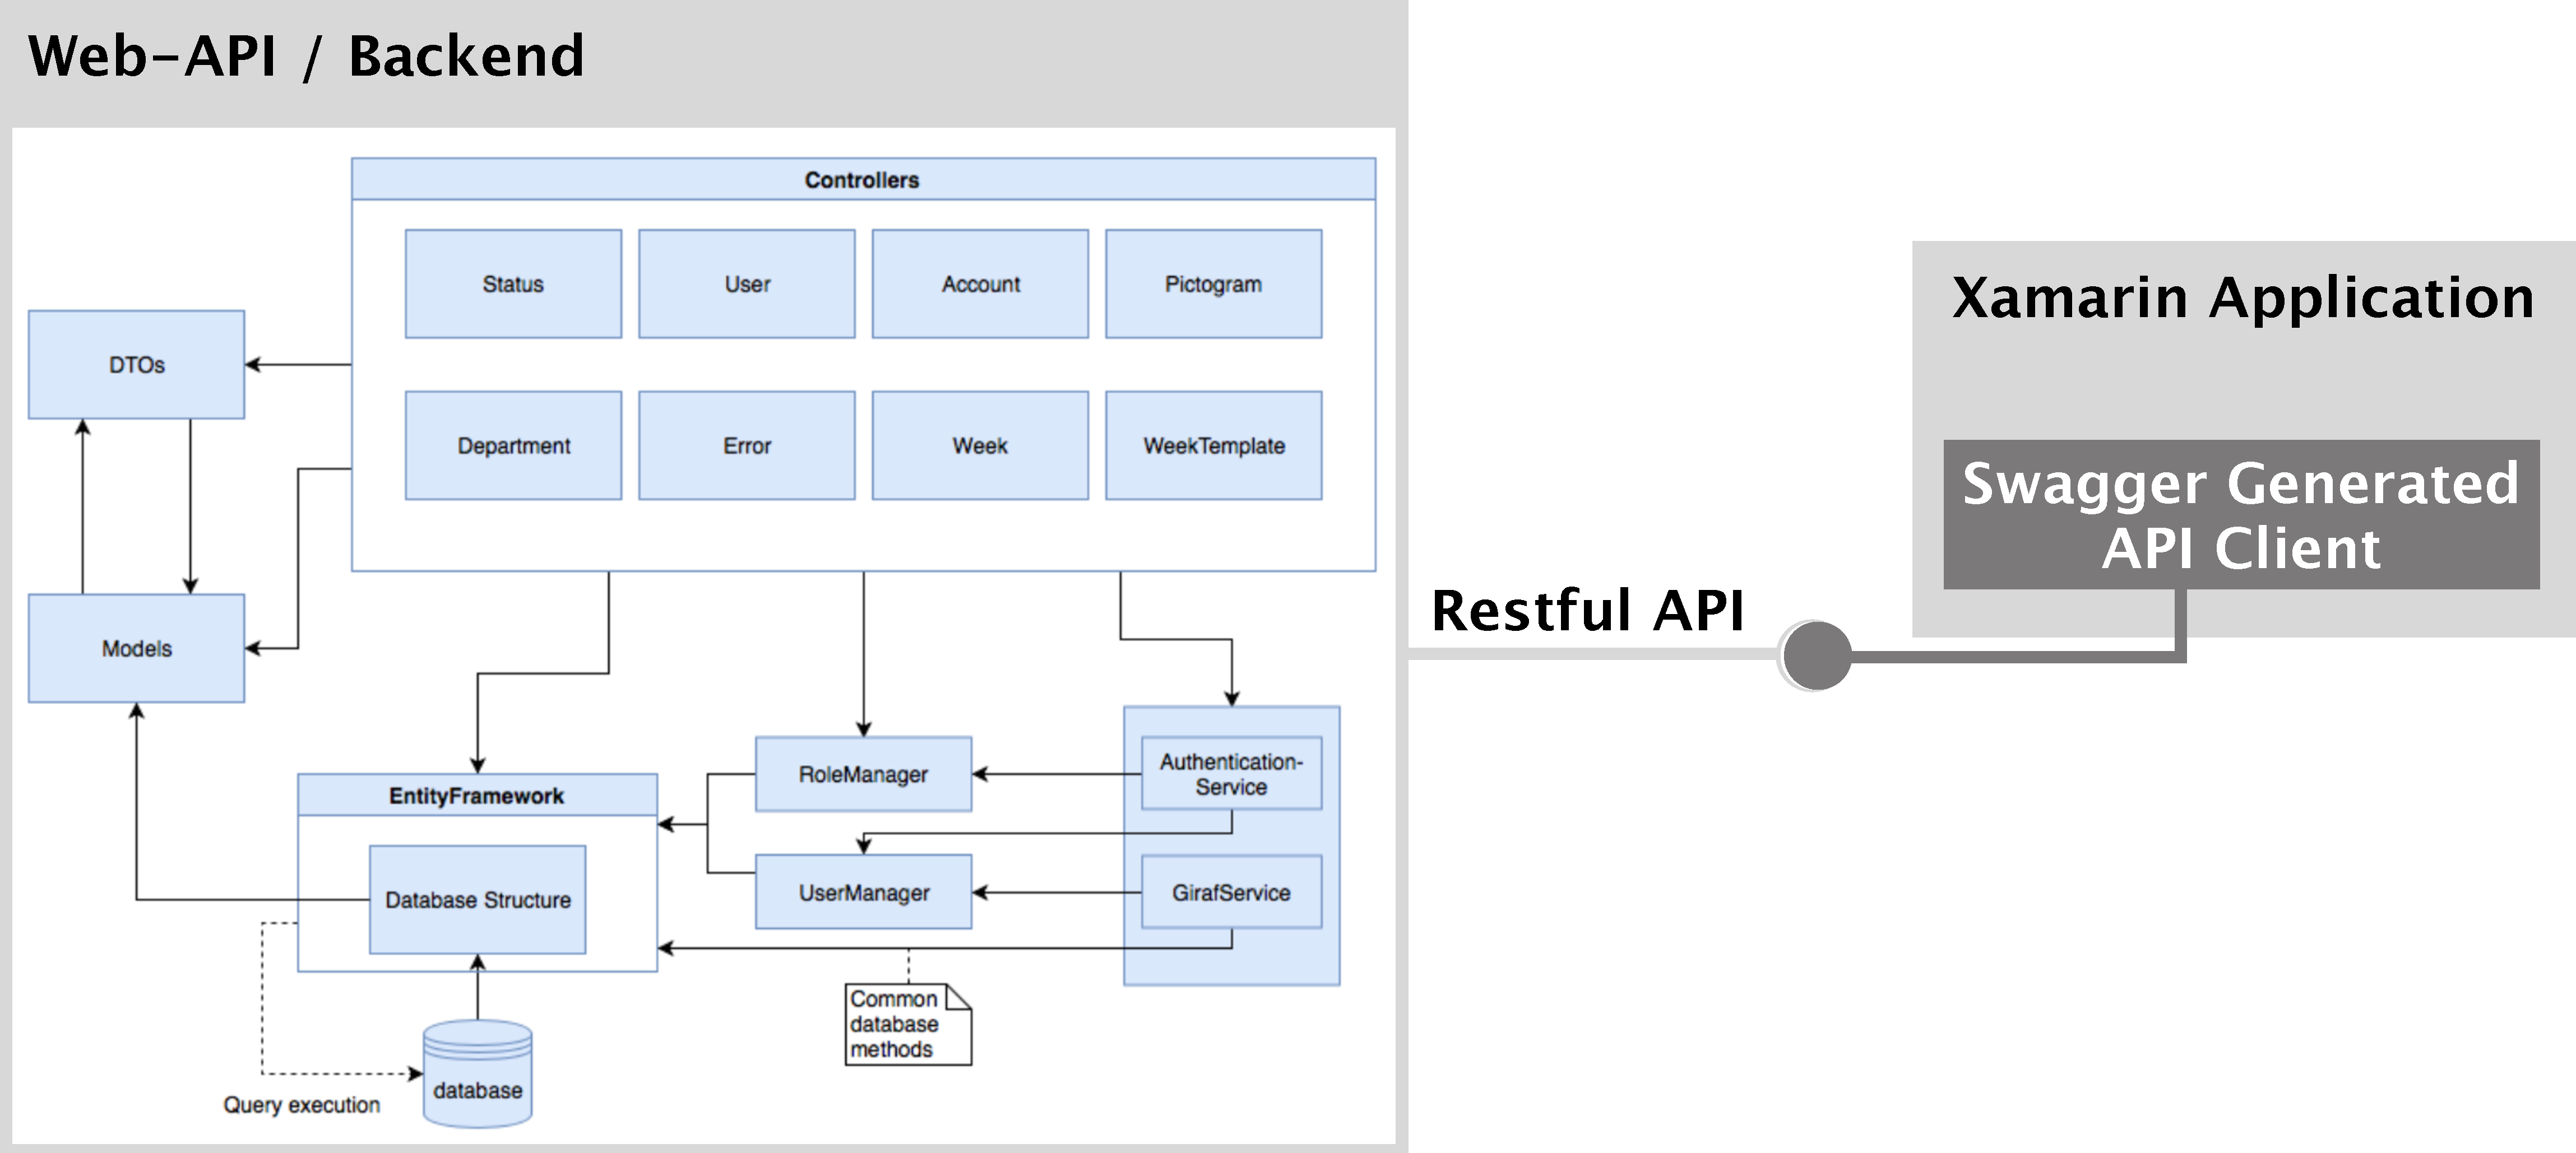
\includegraphics[width=0.95\textwidth]{figures/RestAPIFigure.pdf}
        \end{center}
        \caption{Illustration of the .NET Core 2 project and how it exposes a RESTful API}
        \label{fig:RestAPIFigure}
\end{figure}

